\documentclass[12pt]{article}%全局正文字体为小四

\usepackage{CUMCMPackage}
%\usepackage[nolinenum]{CUMCMPackage} %插入代码不加行号
%\usepackage[TeXLive]{CUMCMPackage} %插入代码不加行号

\problem{A}
\teamNum{27004027}
\Myschool{西安电子科技大学}
\Mymember{队\quad 长}{队\quad 员}{队\quad 员}
\supervisor{教练组}

\title{测试文档}

\begin{document}
\begin{abstract}
这里是摘要,是对文章的高度概括,书写请尽量突出文章的亮点,篇幅不宜过长,绝对不要超过一页(也没人会蠢到这么干-\_-|||)
\begin{keywords}
    关键词1\quad 关键词2 \quad 关键词3
\end{keywords}
\end{abstract}

\maketitle
%\newpage
%\tableofcontents%目录%国赛中是不需要目录的

\newpage
\section{问题重述}


\section{问题分析}
\subsection{问题一的分析}
\subsubsection{呵呵}
字体对否???


\section{模型假设}
\begin{enumerate}
\item 假设无特殊环境影响
\end{enumerate}

\section{符号说明}
\begin{center}
\begin{tabular}{C{3cm} L{8cm}}%r 表示表格内文本右对齐;c表示居中对齐;l表示左对齐;| 表示竖铅直线
    \toprule[2pt]
    \textbf{符号} & \makecell[c]{\textbf{说明}}\\
    \hline
    $\sigma$ & The standard deviation\\
    110010101010 & binary \\
    $\mathbf{F}$ & This is the most beautiful symbol. \\
    \bottomrule[2pt]
\end{tabular}
\end{center}
\textbf{注:}其他符号的说明会在下文中给出。
\section{模型建立与求解}

\begin{figure}[!h]
\centering
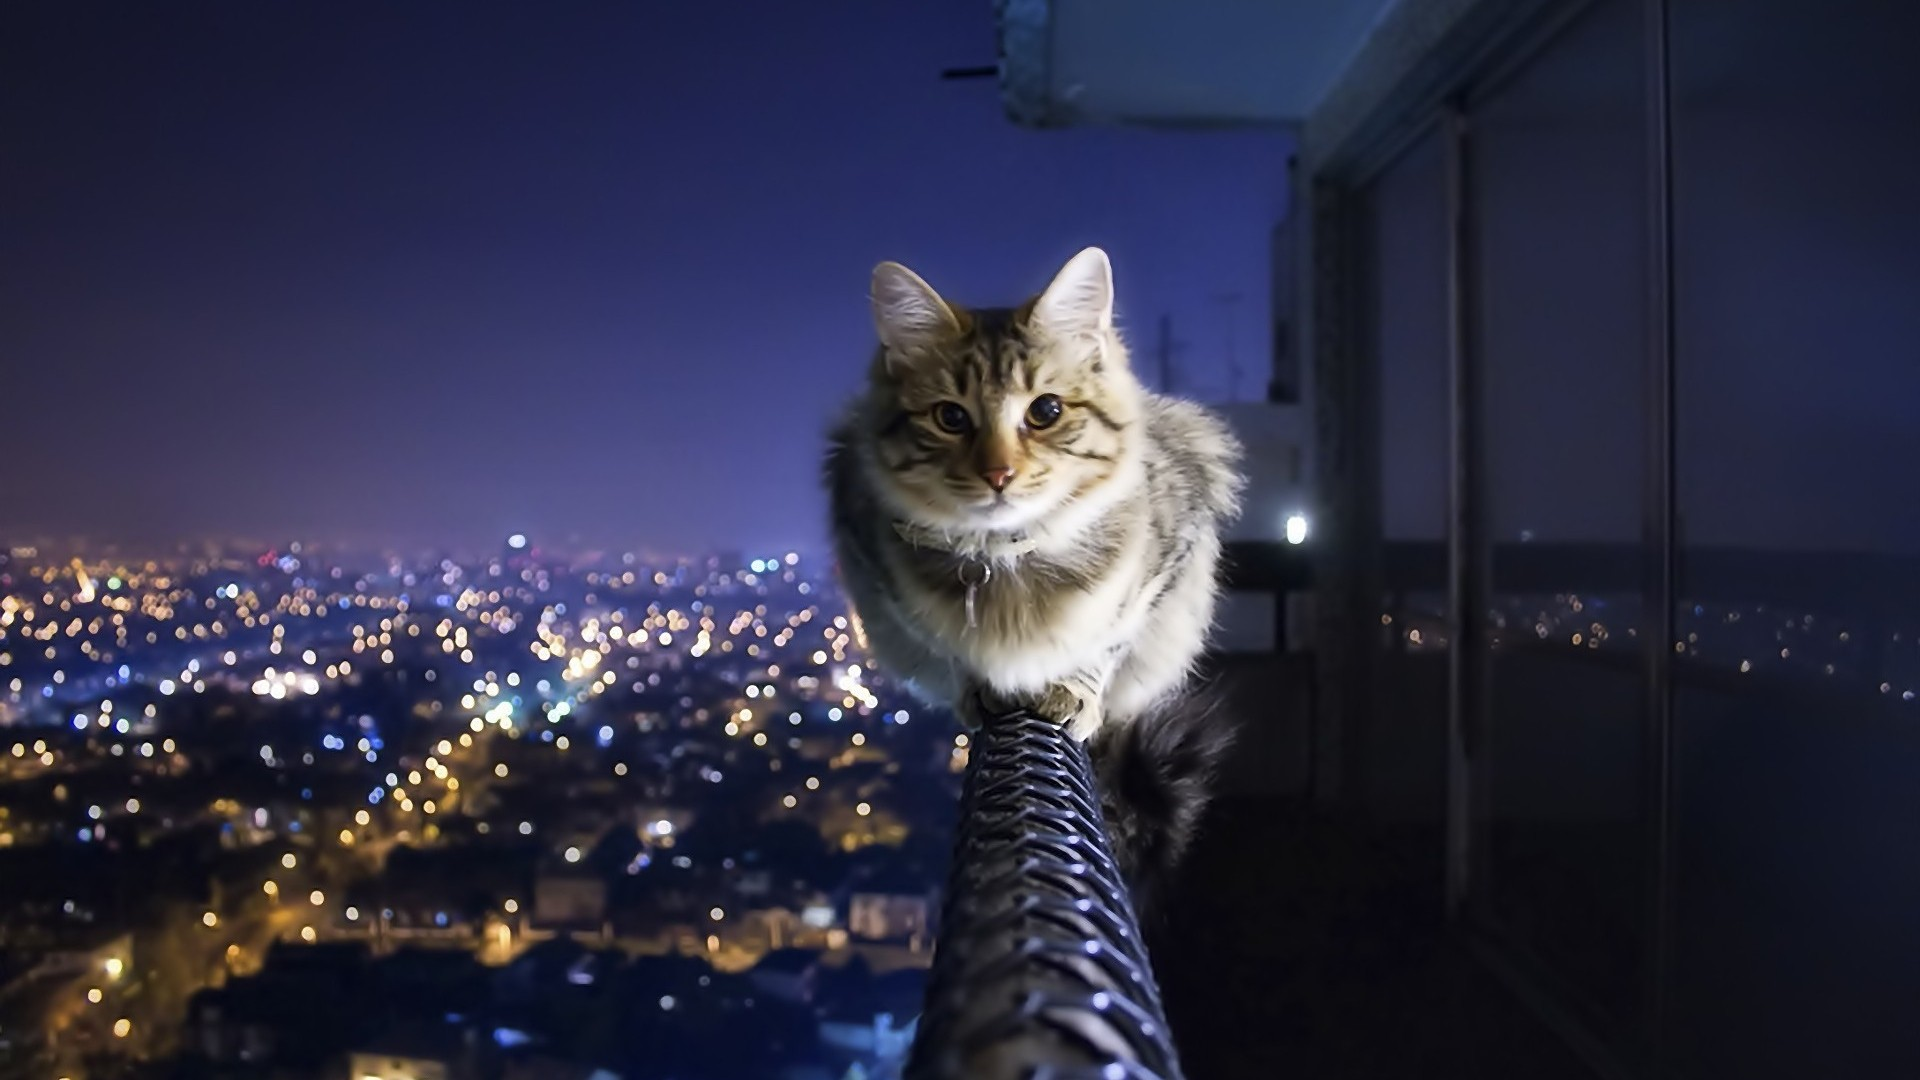
\includegraphics[width=0.7\textwidth]{./Image/testFigure.jpg}
\caption{测试图片1}
\end{figure}

\begin{figure}[!h]
\centering
\begin{minipage}[t]{0.4\linewidth}
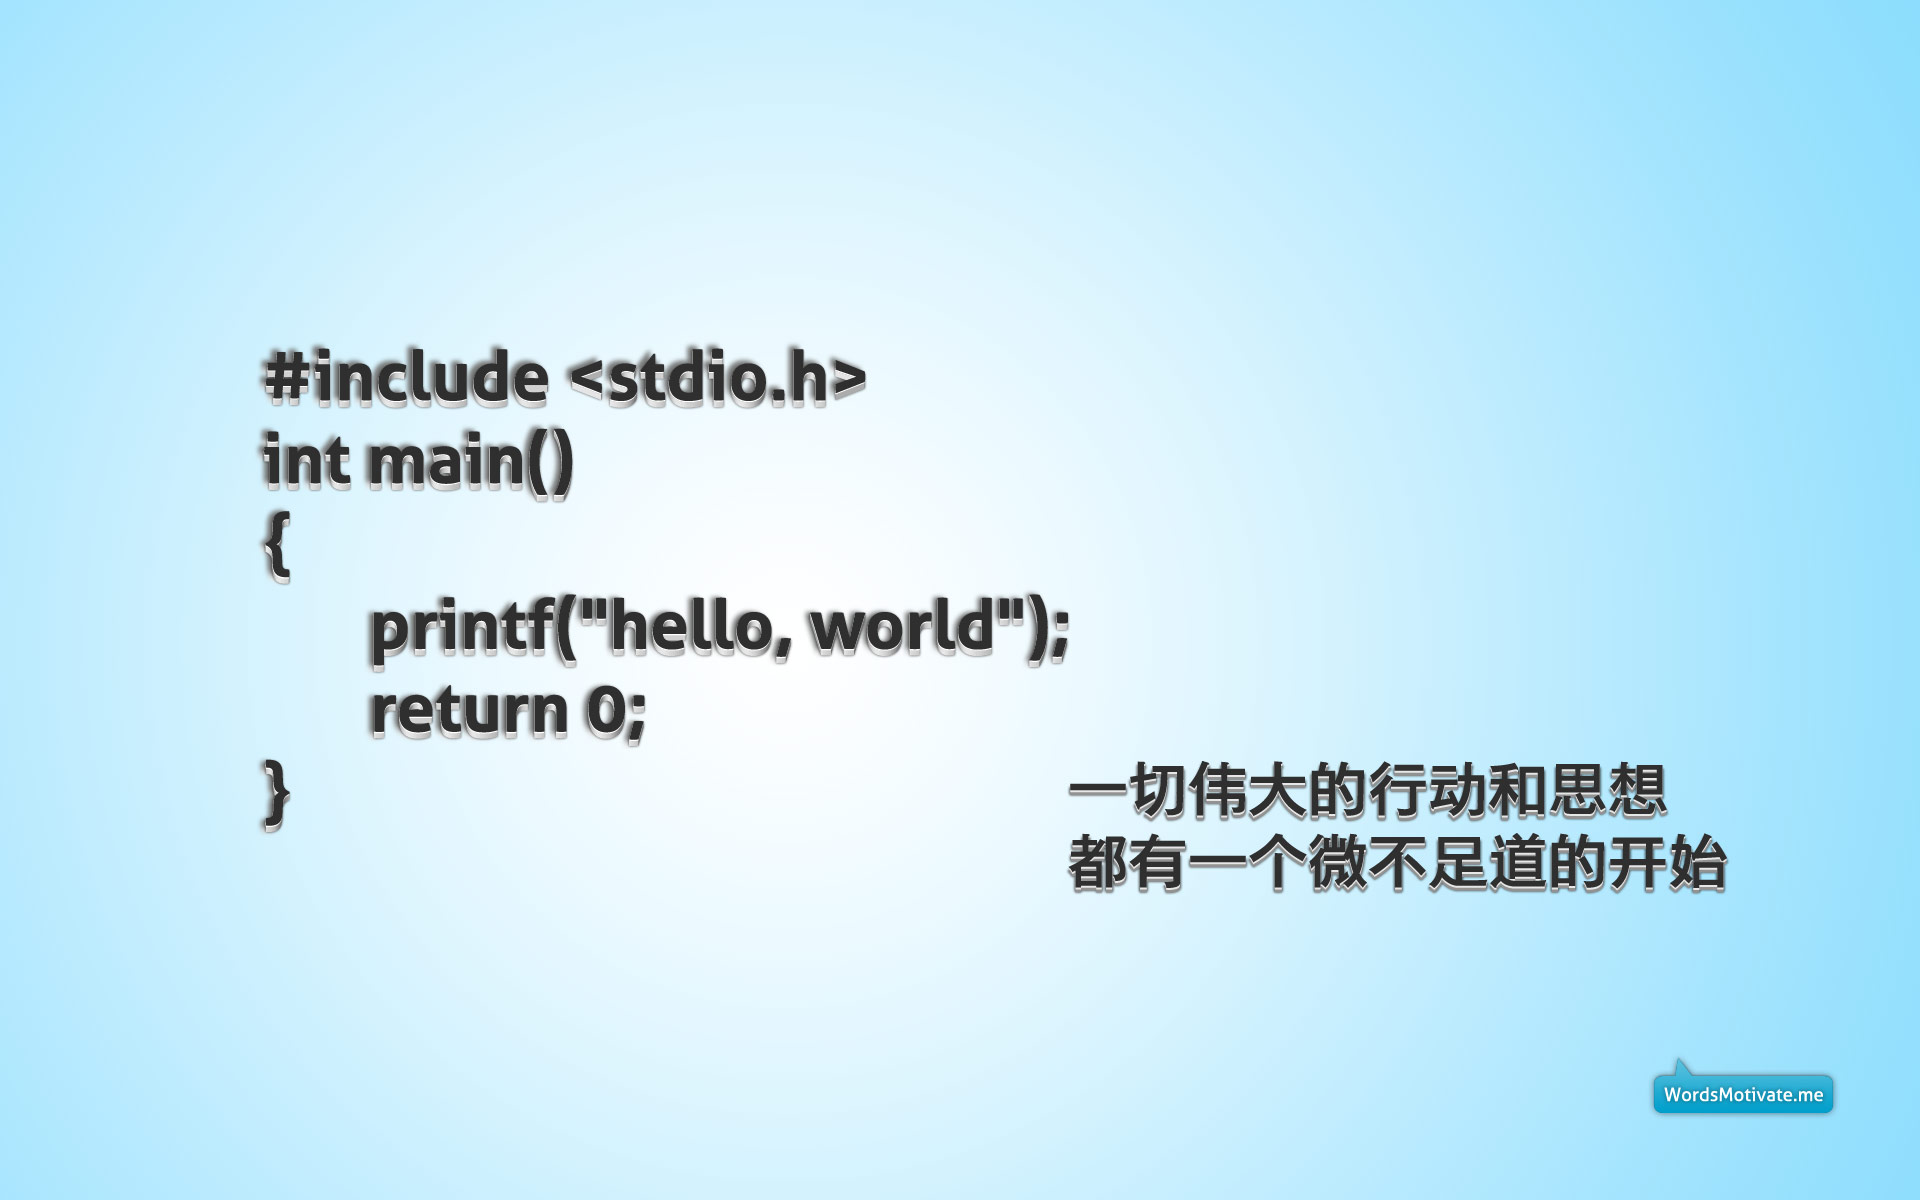
\includegraphics[width=\textwidth]{./Image/zuhe1.jpg}
\end{minipage}~~
\begin{minipage}[t]{0.4\linewidth}

\includegraphics[width=\textwidth]{./Image/zuhe2.jpg}
\end{minipage}
\caption{测试图片2}
\end{figure}
\section{模型分析与评价}

表格测试
\begin{table}[!h]
\centering
\caption{测试表格}
\begin{tabular}{C{4cm}|>{\columncolor{yellow}}C{4cm}}
\toprule[1pt]
\textbf{左标题} & \textbf{右标题}\\
\hline
1 & 一\\
\cellcolor[rgb]{.9,.9,.9} 2 & 二\\
\cellcolor[rgb]{.2,.9,.9} 3 & 三\\
\bottomrule[1pt]
\end{tabular}
\end{table}

\section{模型推广}

行内部公式:$ \theta=\frac{\pi}{3} $

不标号公式
\[S=\sum_{i=1}^{N}\sin{\theta}\]

\begin{equation}
S=\sum_{i=1}^{N}\sin{\theta}
\end{equation}

\begin{equation}
\left\{
   \begin{aligned}
   &c_{i1}=\frac{(x_i,y_1)}{\sqrt{\sum_{j=1}^{n}y_{1j}^2}}\\
   &c_{i2}=\frac{(x_i,y_2)}{\sqrt{\sum_{j=1}^{n}y_{2j}^2}}\\
   &c_{i3}=\frac{(x_i,y_3)}{\sqrt{\sum_{j=1}^{n}y_{3j}^2}}\\
   \end{aligned}
   \right.
\end{equation}

\[
\left( {\begin{array}{*{20}c}
   {a_{11}} & {a_{12}} & {a_{13}}  \\
   {a_{21}} & {a_{22}} & {a_{23}}  \\
   {a_{31}} & {a_{32}} & {a_{33}}  \\
\end{array}} \right) = \frac{{Opposite}}{{Hypotenuse}}\cos ^{ - 1} \theta \arcsin \theta
\]
\section{参考文献的引用}
\noindent 以下参考文献与原有plain风格内容并无再添加

期刊\cite{Art},专著(无页码)\cite{Boo},专著(含页码)\cite{InBoo},论文集\cite{Incol}。

$\newline$

\noindent 以下参考文献相比原有plain风格,内容上再添加了页码项

硕士\cite{MT}/博士论文\cite{Phd},科技报告\cite{TechR}。

$\newline$

\noindent 以下参考文献,原有plain风格中并无,为Stick本人自己写的。

网络内容引用\cite{Net},译著\cite{Trans}

%以下是参考文献
\phantomsection%生成该页的链接
\addcontentsline{toc}{section}{\refname}%将附录添加到目录中,如果不想在目录中看到可以连同上面的一行代码一起注释掉
\bibliographystyle{RefWithChSty}%plain ieeetr
\bibliography{RefFile}%在正文中必须引用,才能显示对应的参考文献

%\phantomsection%生成该页的链接
%\addcontentsline{toc}{section}{\refname}%将附录添加到目录中,如果不想在目录中看到可以连同上面的一行代码一起注释掉
%\begin{thebibliography}{}
%%
%% 使用指令\bibitem 构造一条参考文献.
%% 具体构造方式,参考以下参考文献格式说明以及示例
%%
%\bibitem{RefJ}
%% 期刊引用格式
%    % 中文的引用格式
%    % 作者. 标题[J].期刊名, 发表年份,  卷号(期号), 页码
%	王晓晨,潘晨,五轩. 十问嫦娥——揭秘嫦娥三号探测器[J]. 中国航天纪念专刊, 2014,(1):15-26
%
%\bibitem{RefB}
%% 书本/专著引用格式
%    % 中文的引用格式
%    % 作者名. 书名[M]. 出版地: 出版社, 出版年份: 页码.
%	姜启源,谢金星,叶俊. 数学模型(第四版)[M]. 北京:高等教育出版社,2011.
%% etc
%\end{thebibliography}

\newpage
%在正文中添加附录
\begin{appendices}
真的是这样子的吗???\CJKnumber{12345}
\begin{subappendix}
子附录测试

\codetitle{Matlab代码}
\lstinputlisting[language=Matlab]{./Code/AHPtest.m}

\codetitle{R代码}
\lstinputlisting[language=R]{./Code/example.R}

\end{subappendix}

\begin{subappendix}
子附录测试2
\end{subappendix}

\begin{subappendix}
子附录测试3

\centerline{\sihao\color{red}千字文}
\begin{center}
天地玄黄 (tiān dì xuán huáng),宇宙洪荒 (yǔ zhòu hóng huāng)。

日月盈昃 (rì yuè yíng zè),辰宿列张 (chén xiù liè zhāng)。

寒来暑往 (hán lái shǔ wǎng),秋收冬藏 (qiū shōu dōng cáng)。

闰余成岁 (rùn yú chéng suì), 律吕调阳 (lǜ lǚ tiáo yáng)。

云腾致雨 (yún téng zhì yǔ), 露结为霜 (lù jié wéi shuāng)。

金生丽水 (jīn shēng lì shuǐ), 玉出昆冈 (yù chū kūn gāng)。

剑号巨阙 (jiàn hào jù què), 珠称夜光 (zhū chēng yè guāng)。

果珍李柰 (guǒ zhēn lǐ nài), 菜重芥姜 (cài zhòng jiè jiāng)。

海咸河淡 (hǎi xián hé dàn), 鳞潜羽翔 (lín qián yǔ xiáng)。

龙师火帝 (lóng shī huǒ dì), 鸟官人皇 (niǎo guān rén huáng)。

始制文字 (shǐ zhì wén zì), 乃服衣裳 (nǎi fú yī shāng)。

推位让国 (tuī wèi ràng guó), 有虞陶唐 (yǒu yú táo táng)。

吊民伐罪 (diào mín fá zuì), 周发殷汤 (zhōu fā yīn tāng)。

坐朝问道 (zuò cháo wèn dào), 垂拱平章 (chuí gǒng píng zhāng)。

爱育黎首 (ài yù lí shǒu), 臣伏戎羌 (chén fú róng qiāng)。

遐迩一体 (xiá ěr yī tǐ), 率宾归王 (shuài bīn guī wáng)。

鸣凤在竹 (míng fèng zài zhú), 白驹食场 (bái jū shí chǎng)。

化被草木 (huà bèi cǎo mù), 赖及万方 (lài jí wàn fāng)。

盖此身发 (gài cǐ shēn fà), 四大五常 (sì dà wǔ cháng)。

恭惟鞠养 (gōng wéi jū yǎng), 岂敢毁伤 (qǐ gǎn huǐ shāng)。

女慕贞洁 (nǚ mù zhēn jié), 男效才良 (nán xiào cái liáng)。

知过必改 (zhī guò bì gǎi), 得能莫忘 (dé néng mò wàng)。

罔谈彼短 (wǎng tán bǐ duǎn), 靡恃己长 (mí shì jǐ cháng)。

信使可覆 (xìn shǐ kě fù), 器欲难量 (qì yù nán liáng)。

墨悲丝染 (mò bēi sī rǎn), 诗赞羔羊 (shī zàn gāo yáng)。

景行维贤 (jǐng xíng wéi xián), 克念作圣 (kè niàn zuò shèng)。

德建名立 (dé jiàn míng lì), 形端表正 (xíng duān biǎo zhèng)。

空谷传声 (kōng gǔ chuán shēng), 虚堂习听 (xū táng xí tīng)。

祸因恶积 (huò yīn è jí), 福缘善庆 (fú yuán shàn qìng)。

尺璧非宝 (chǐ bì fēi bǎo), 寸阴是竞 (cùn yīn shì jìng)。

资父事君 (zī fù shì jūn), 曰严与敬 (yuē yán yǔ jìng)。

孝当竭力 (xiào dāng jié lì), 忠则尽命 (zhōng zé jìn mìng)。

临深履薄 (lín shēn lǚ báo), 夙兴温凊 (sù xīng wēn qìng)。

似兰斯馨 (sì lán sī xīn), 如松之盛 (rú sōng zhī shèng)。

川流不息 (chuān liú bù xī), 渊澄取映 (yuān chéng qǔ yìng)。

容止若思 (róng zhǐ ruò sī), 言辞安定 (yán cí ān dìng)。

笃初诚美 (dǔ chū chéng měi), 慎终宜令 (shèn zhōng yì lìng)。

荣业所基 (róng yè suǒ jī), 籍甚无竟 (jí shèn wú jìng)。

学优登仕 (xué yōu dēng shì), 摄职从政 (shè zhǐ cóng zhèng)。

存以甘棠 (cún yǐ gān táng), 去而益咏 (qù ér yì yǒng)。

乐殊贵贱 (yuè shū guì jiàn), 礼别尊卑 (lǐ bié zūn bēi)。

上和下睦 (shàng hé xià mù), 夫唱妇随 (fū chàng fù suí)。

外受傅训 (wài shòu fù xùn), 入奉母仪 (rù fèng mǔ yí)。

诸姑伯叔 (zhū gū bó shú), 犹子比儿 (yōu zǐ bǐ ér)。

孔怀兄弟 (kǒng huái xiōng dì), 同气连枝 (tóng qì lián zhī)。

交友投分 (jiāo yǒu tóu fēn), 切磨箴规 (qiē mó zhēn guī)。

仁慈隐恻 (rén cí yǐn cè), 造次弗离 (zào cì fú lí)。

节义廉退 (jié yì lián tuì),颠沛匪亏 (diān pèi fěi kuī)。

性静情逸 (xìng jìng qíng yì),心动神疲 (xīn dòng shén pí)。

守真志满 (shǒu zhēn zhì mǎn),逐物意移 (zhú wù yì yí)。

坚持雅操 (jiān chí yǎ cāo),好爵自縻 (hǎo jué zì mí)。

都邑华夏 (dū yì huá xià),东西二京 (dōng xī èr jīng)。

背邙面洛 (bèi máng miàn luò),浮渭据泾 (fú wèi jù jīng)。

宫殿盘郁 (gōng diàn pán yù),楼观飞惊 (lóu guàn fēi jīng)。

图写禽兽 (tú xiě qín shòu),画彩仙灵 (huà cǎi xiān líng)。

丙舍旁启 (bǐng shè páng qǐ),甲帐对楹 (jiǎ zhàng duì yíng)。

肆筵设席 (sì yán shè xí),鼓瑟吹笙 (gǔ sè chuī shēng)。

升阶纳陛 (shēng jiē nà bì),弁转疑星 (biàn zhuàn yí xīng)。

右通广内 (yòu tōng guǎng nèi),左达承明 (zuǒ dá chéng míng)。

既集坟典 (jì jí fén diǎn),亦聚群英 (yì jù qún yīng)。

杜稿钟隶 (dù gǎo zhōng lì),漆书壁经 (qī shū bì jīng)。

府罗将相 (fǔ luó jiàng xiàng),路侠槐卿 (lù jiā huái qīng)。

户封八县 (hù fēng bā xiàn),家给千兵 (jiā jǐ qiān bīng)。

高冠陪辇 (gāo guān péi niǎn),驱毂振缨 (qū gǔ zhèn yīng)。

世禄侈富 (shì lù chǐ fù),车驾肥轻 (chē jià féi qīng)。

策功茂实 (cè gōng mào shí),勒碑刻铭 (lè bēi kè míng)。

磻溪伊尹 (pán xī yī yǐn),佐时阿衡 (zuǒ shí ē héng)。

奄宅曲阜 (yǎn zhái qū fù),微旦孰营 (wēi dàn shú yíng)。

桓公匡合 (huán gōng kuāng hé), 济弱扶倾 (jì ruò fú qīng)。

绮回汉惠 (qǐ huí hàn huì), 说感武丁 (yuè gǎn wǔ dīng)。

俊乂密勿 (jùn yì mì wù), 多士实宁 (duō shì shí níng)。

晋楚更霸 (jìn chǔ gēng bà), 赵魏困横 (zhào wèi kùn héng)。

假途灭虢 (jiǎ tú miè guó), 践土会盟 (jiàn tǔ huì méng)。

何遵约法 (hé zūn yuē fǎ), 韩弊烦刑 (hán bì fán xíng)。

起翦颇牧 (qǐ jiǎn pō mù), 用军最精 (yòng jūn zuì jīng)。

宣威沙漠 (xuān wēi shā mò), 驰誉丹青 (chí yù dān qīng)。

九州禹迹 (jiǔ zhōu yǔ jì), 百郡秦并 (bǎi jùn qín bìng)。

岳宗泰岱 (yuè zōng tài dài), 禅主云亭 (shàn zhǔ yún tíng)。

雁门紫塞 (yàn mén zǐ sài), 鸡田赤城 (jī tián chì chéng)。

昆池碣石 (kūn chí jié shí), 钜野洞庭 (jù yě dòng tíng)。

旷远绵邈 (kuàng yuǎn mián miǎo), 岩岫杳冥 (yán xiù yǎo míng)。

治本于农 (zhì běn yú nóng), 务兹稼穑 (wù zī jià sè)。

俶载南亩 (chù zǎi nán mǔ), 我艺黍稷 (wǒ yì shǔ jì)。

税熟贡新 (shuì shú gòng xīn), 劝赏黜陟 (quàn shǎng chù zhì)。

孟轲敦素 (mèng kē dūn sù), 史鱼秉直 (shǐ yú bǐng zhí)。

庶几中庸 (shù jǐ zhōng yōng), 劳谦谨敕 (láo qiān jǐn chì)。

聆音察理 (líng yīn chá lǐ), 鉴貌辨色 (jiàn mào biàn sè)。

贻厥嘉猷 (yí jué jiā yóu), 勉其祗植 (miǎn qí zhī zhí)。

省躬讥诫 (xǐng gōng jī jiè), 宠增抗极 (chǒng zēng kàng jí)。

殆辱近耻 (dài rǔ jìn chǐ), 林皋幸即 (lín gāo xìng jí)。

两疏见机 (liǎng shū jiàn jī), 解组谁逼 (jiè zǔ shuí bī)。

索居闲处 (suǒ jū xián chǔ), 沉默寂寥 (chén mò jì liào)。

求古寻论 (qiú gǔ xún lùn), 散虑逍遥 (sǎn lǜ xiāo yáo)。

欣奏累遣 (xīn zòu lèi qiǎn), 戚谢欢招 (qī xiè huān zhāo)。

渠荷的历 (qú hé dì lì), 园莽抽条 (yuán mǎng chōu tiáo)。

枇杷晚翠 (pí pá wǎn cuì), 梧桐蚤凋 (wú tóng zǎo diāo)。

陈根委翳 (chén gēn wěi yì), 落叶飘摇 (luò yè piāo yáo)。

游鹍独运 (you kūn dú yùn), 凌摩绛霄 (líng mó jiàng xiāo)。

耽读玩市 (dān dú wán shì), 寓目囊箱 (yù mù náng xiāng)。

易輶攸畏 (yì yóu yōu wèi), 属耳垣墙 (zhǔ ěr yuán qiáng)。

具膳餐饭 (jù shàn cān fàn), 适口充肠 (shì kǒu chōng cháng)。

饱饫烹宰 (bǎo yù pēng zǎi), 饥厌糟糠 (jī yàn zāo kāng)。

亲戚故旧 (qīn qì gù jiù), 老少异粮 (lǎo shào yì liáng)。

妾御绩纺 (qiè yù jì fǎng), 侍巾帷房 (shì jīn wéi fáng)。

纨扇圆洁 (wán shàn yuán jié), 银烛炜煌 (yín zhú wěi huáng)。

昼眠夕寐 (zhòu mián xī mèi), 蓝笋象床 (lán sǔn xiàng chuáng)。

弦歌酒宴 (xián gē jiǔ yàn), 接杯举觞 (jié bēi jǔ shāng)。

矫手顿足 (jiǎo shǒu dùn zú), 悦豫且康 (yuè yù qiě kāng)。

嫡后嗣续 (dí hòu sì xù), 祭祀烝尝 (jì sì zhēng cháng)。

稽颡再拜 (jī sǎng zài bài), 悚惧恐惶 (sǒng jù kǒng huáng)。

笺牒简要 (jiān dié jiǎn yào), 顾答审详 (gù dá shěn xiáng)。

骸垢想浴 (hài gòu xiǎng yù), 执热愿凉 (zhí rè yuàn liáng)。

驴骡犊特 (lǘ luó dú tè), 骇跃超骧 (hài yuè chāo xiāng)。

诛斩贼盗 (zhū zhǎn zéi dào), 捕获叛亡 (pǔ huò pàn wáng)。

布射僚丸 (bù shè liáo wán), 嵇琴阮啸 (jī qín ruǎn xiào)。

恬笔伦纸 (tián bǐ lún zhǐ), 钧巧任钓 (jūn qiǎo rén diào)。

释纷利俗 (shì fēn lì sú), 并皆佳妙 (bìng jiē jiā miào)。

毛施淑姿 (máo shī shū zī), 工颦妍笑 (gōng pín yán xiào)。

年矢每催 (niánshǐměicuī), 曦晖朗曜 (xī huī lǎng yào)。

璇玑悬斡 (xuán jī xuán wò), 晦魄环照 (huì pò huán zhào)。

指薪修祜 (zhǐ xīn xiū hù), 永绥吉劭 (yǒng suí jí shào)。

矩步引领 (jù bù yǐn lǐng), 俯仰廊庙 (fǔ yǎng láng miào)。

束带矜庄 (shù dài jīn zhuāng), 徘徊瞻眺 (pái huái zhān tiào)。

孤陋寡闻 (gū lòu guǎ wén), 愚蒙等诮 (yú méng děng qiào)。

谓语助者 (wèi yǔ zhù zhě),焉哉乎也 (yān zāi hū yě)。
\end{center}
\end{subappendix}

\end{appendices}

\end{document}
